\documentclass[12pt]{article}
\usepackage{amsmath}
\usepackage[margin=1in]{geometry}
\usepackage{graphicx}
\graphicspath{ {images/} }
\begin{document}

\begin{center}

\textbf{George Witteman -- Homework 3}

Modeling, Simulation and Analysis\\CS 250, Spring 2018

\end{center}

\begin{enumerate}
  \item \textbf{Have A Ball!}
  \begin{enumerate}
    \setcounter{enumii}{0}
    
  	\item
    	See Figure \ref{fig:1a-1}.
    	\begin{figure}[h!]
  			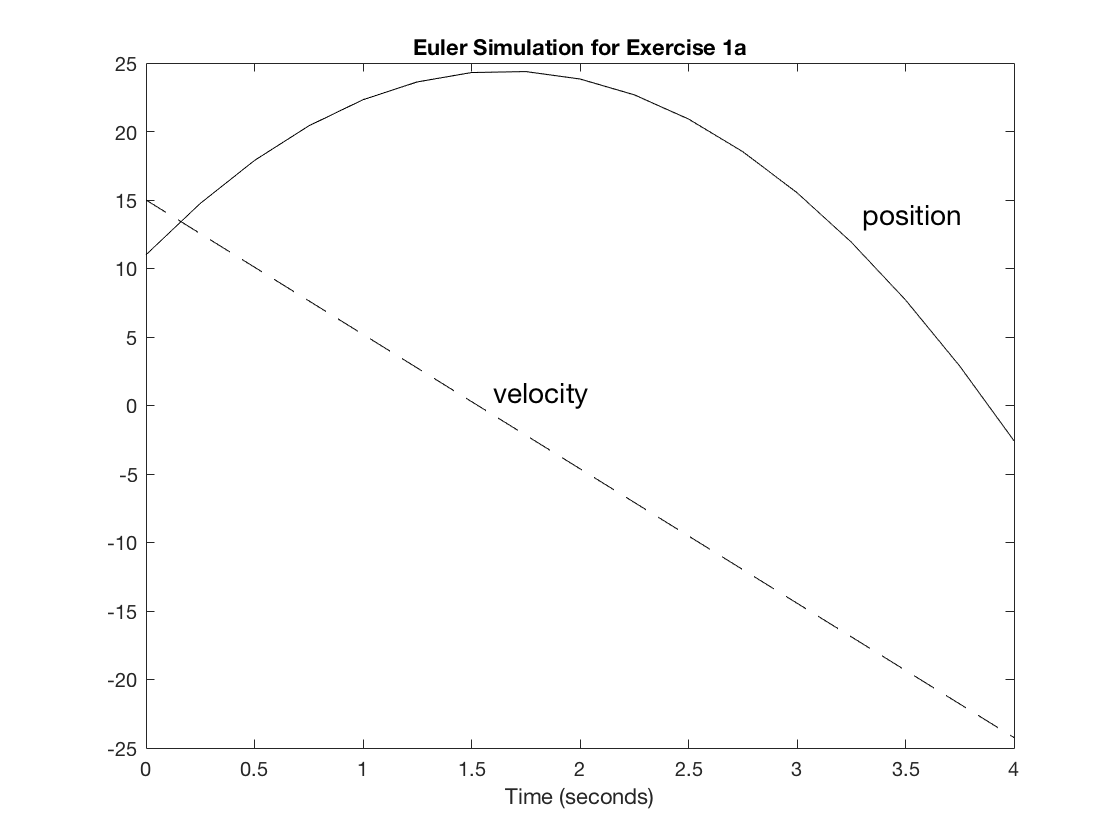
\includegraphics[width=0.666\textwidth]{1a-1}
  			\centering
        \caption{Exercise 1a}
        \label{fig:1a-1}
      \end{figure}
      
    \item
    	See Figure \ref{fig:1b-1}
    	\begin{figure}[h!]
  			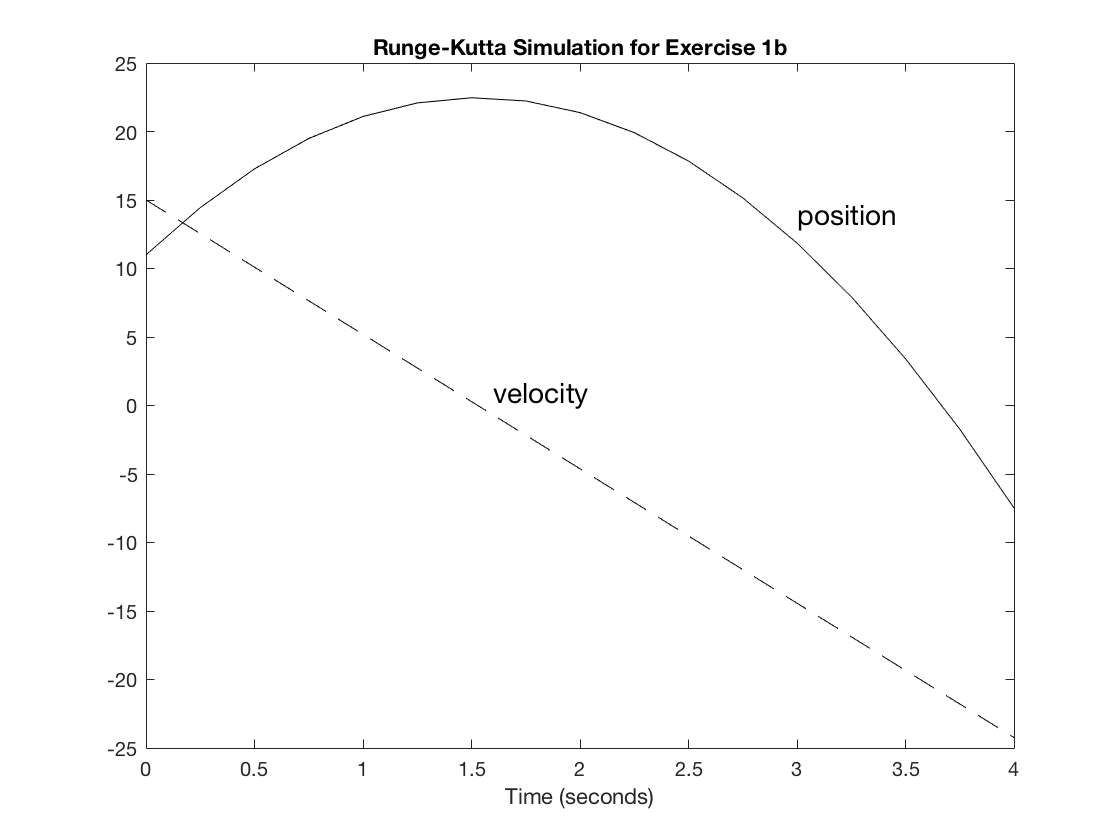
\includegraphics[width=0.666\textwidth]{1b-1}
  			\centering
        \caption{Exercise 1b}
        \label{fig:1b-1}
      \end{figure}
      
    \item
    	See Figure \ref{fig:1c-1}
    	\begin{figure}[h!]
  			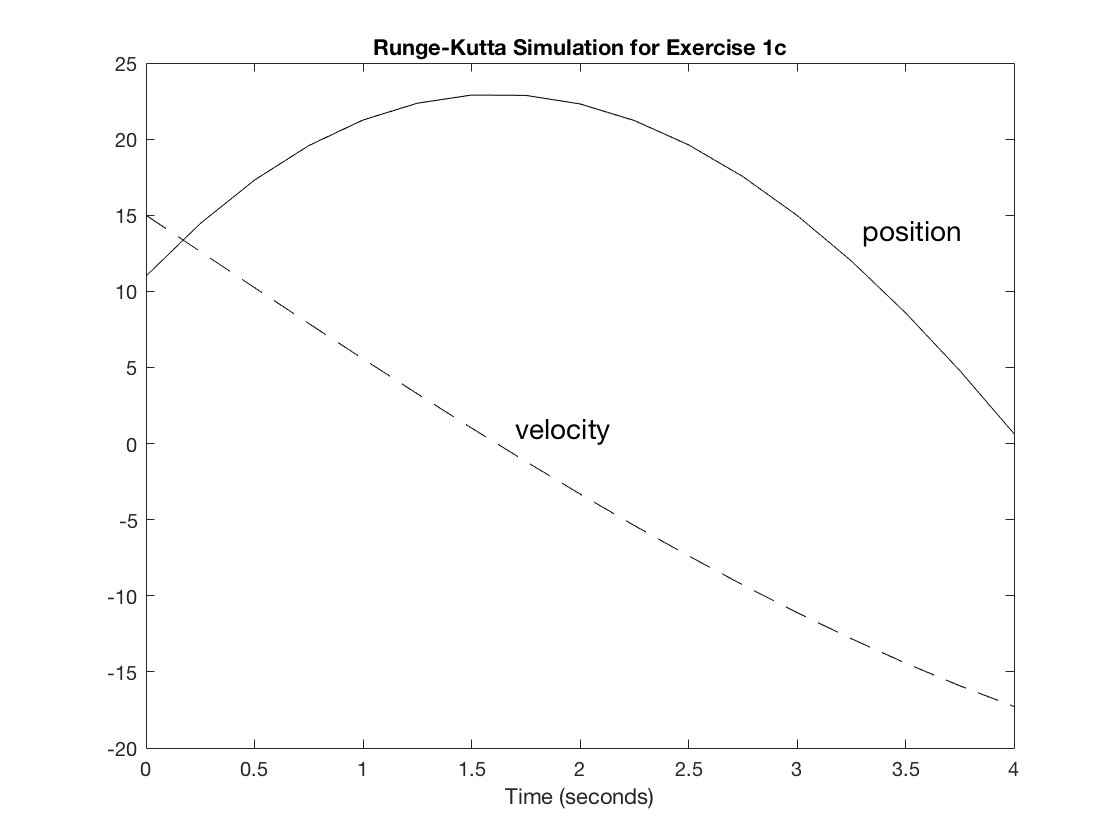
\includegraphics[width=0.666\textwidth]{1c-1}
  			\centering
        \caption{Exercise 1c}
        \label{fig:1c-1}
      \end{figure}
      
     \item
    	 See Figure \ref{fig:1d-1}
    	 \begin{figure}[h!]
  			 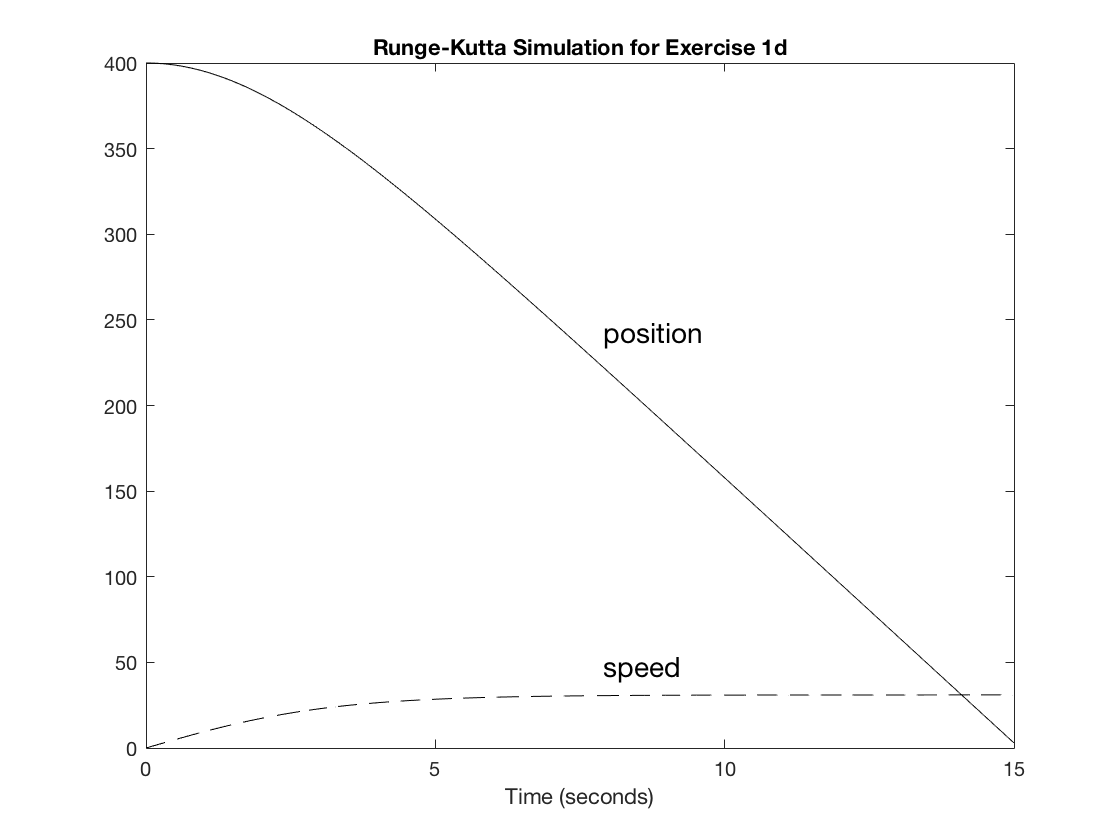
\includegraphics[width=0.666\textwidth]{1d-1}
  			 \centering
         \caption{Exercise 1d}
         \label{fig:1d-1}
       \end{figure}
      
     \item
       The only change needed to convert exercise 1b to exercise 1c is to change the equation for $\frac{dV}{dt}$. In exercise 1c $\frac{dV}{dt}$ is more than just acceleration due to gravity, so I had to change it to $\frac{dV}{dt} = g + 0.01 * (v(t) + h(t)) + 0.3 * t^2$.
       
       In exercise 1d, I first changed the simulation length and $\Delta t$ variables. Then, I added a constant for mass (in kg) and a constant for radius (in meters). The initial position and velocity variables were updated to be 400 and 0 respectively. Finally, the equation for $\frac{dV}{dt}$ was changed to the equation given in the textbook.
       
       For all three of these exercises the simulation loop was able to stay exactly the same by using functions for the differential equations. The only things that needed to change were the equations for those differential equations and any constants that they relied on.
  
  \end{enumerate}
  
  \item \textbf{Brainpower: The Hodgkin-Huxley Model}
  	\begin{enumerate}
	
			\item
  			\begin{figure}[h!]
  			 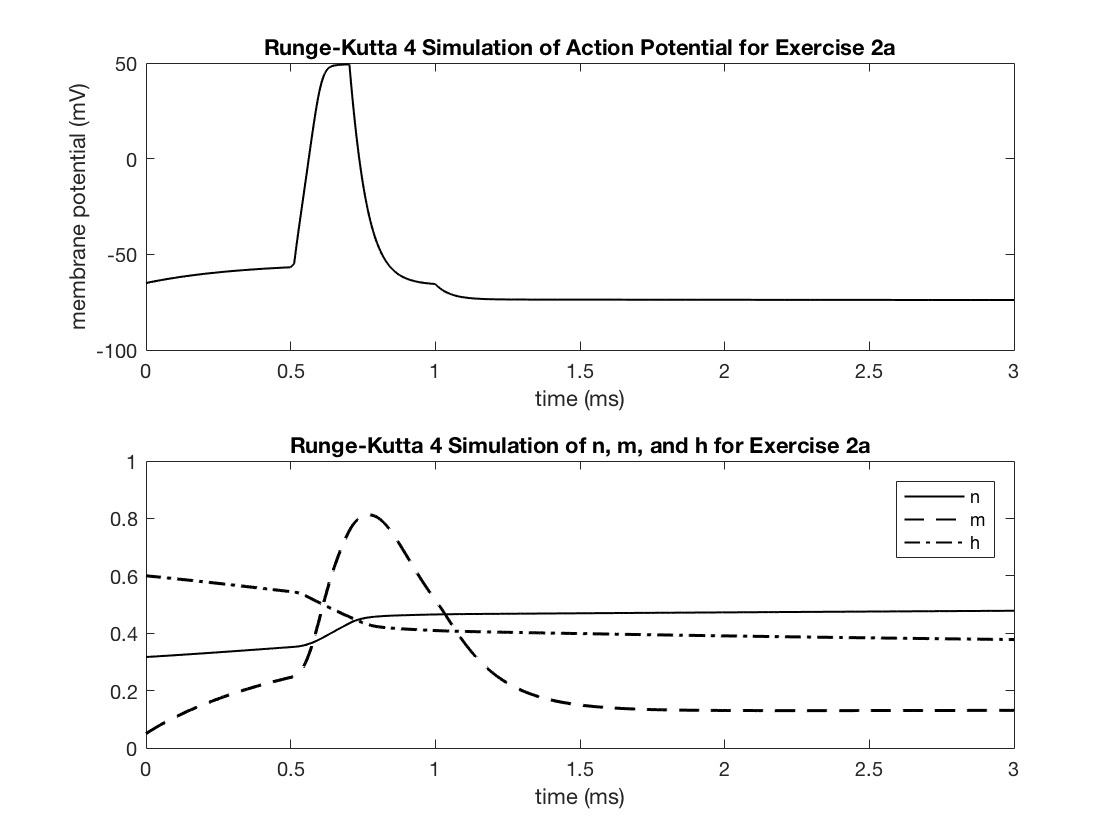
\includegraphics[width=0.666\textwidth]{2a-1}
  			 \centering
         \caption{Exercise 2a}
         \label{fig:2a-1}
       \end{figure}
				See Figure \ref{fig:2a-1}.
				
				This simulation looks similar to the textbook graph. The resting potential phase is similar, but since this version of the model lacks the $Na^+$-$K^+$-ATPase pump it is the $K^+$ ions leak through the membrane without anything to even them out. This results in a slow increase on the voltage of the neuron.
				
				Similar to the textbook graph, there is a spike in the voltage when the action potential begins (i.e. the depolarization phase). Then, once the membrane potential reaches 49.3mV, the action potential enters the repolarization phase. At this point the sodium channel closes and the potassium channel opens. This causes a large number of potassium ions to leave the neuron, decreasing it's membrane potential.
				
				One issue with my model is that it does not leave the hyperpolarization phase. The potassium channel doesn't close when it is supposed to, which causes the potassium channel to always stay open.
				 
			\item
				\begin{figure}[h!]
  			 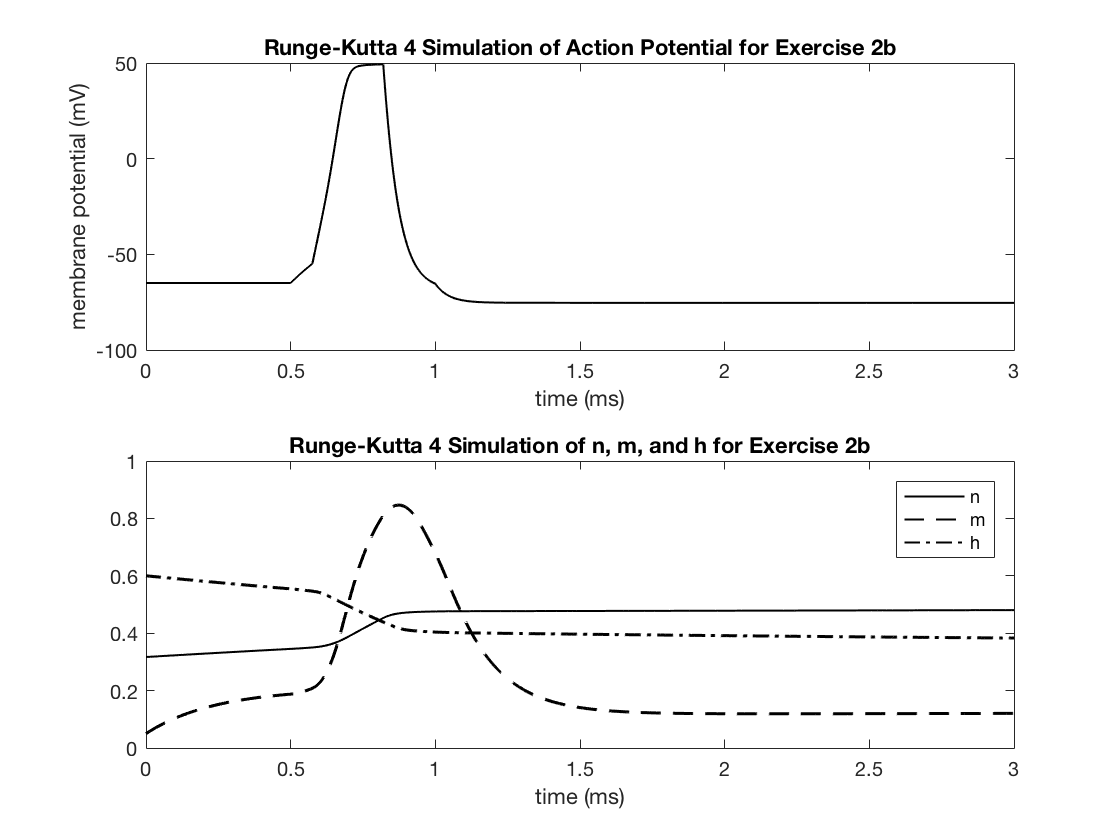
\includegraphics[width=0.666\textwidth]{2b-1}
  			 \centering
         \caption{Exercise 2b}
         \label{fig:2b-1}
       \end{figure}
				See Figure \ref{fig:2b-1}.
				
				There is one main difference between this graph and the graph in exercise 2a. The difference with this graph and 2a is that this graph has a stable resting potential before 0.5ms. This is because the $Na^+$-$K^+$-ATPase pump counteracts the flow of $K^+$ ions in the leakage channel. It removes potassium ions out of the neuron at the same rate that ions leak into the neuron. Therefore, we can conclude that this pump is what allows the resting potential to stay stable and to not have sporadic action potentials.
			
			\item
				\begin{figure}[h!]
  			 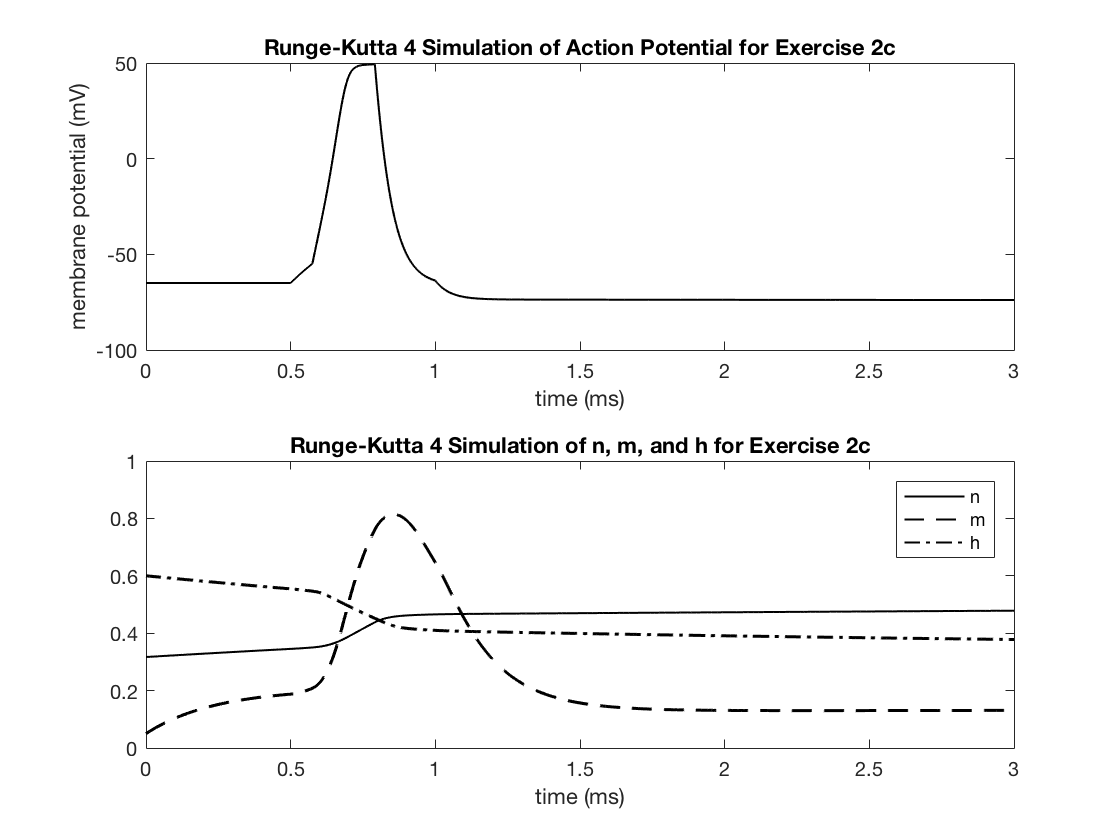
\includegraphics[width=0.666\textwidth]{2c-1}
  			 \centering
         \caption{Exercise 2c}
         \label{fig:2c-1}
       \end{figure}
				See Figure \ref{fig:2c-1}.
				
				The biggest change to this model from the previous models is that we are now keeping track of the concentration of [$Na^+$] and [$K^+$] ions. This is done by finding the change in the concentration of each ion, and adding or subtracting the change to the concentrations on each side of the membrane for each ion.
				
				Since the pump turns off when the concentrations are less than 0, my model will turn off the pump around when the action potential reaches it's peak. I chose to not implement a mechanism to prevent negative values of the concentrations for simplicity of the implementation. This does, however, sacrifice some accuracy, since the pump doesn't turn on again after the concentrations reach 0. 
				
			\item
				\begin{figure}[h!]
  			 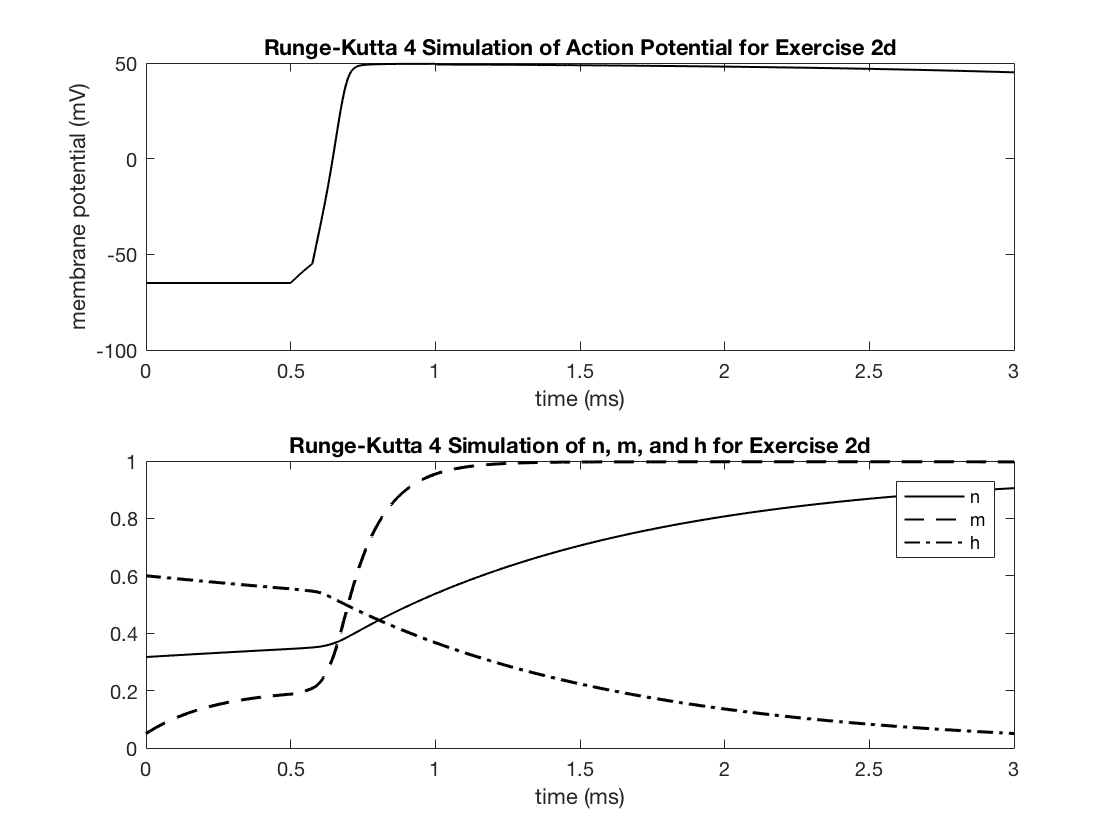
\includegraphics[width=0.666\textwidth]{2d-1}
  			 \centering
         \caption{Exercise 2d}
         \label{fig:2d-1}
       \end{figure}
				See Figure \ref{fig:2d-1}.
				
				With this simulation, the sodium gates never close because the threshold for the sodium channel to close (50mV) is never reached. Since it never closes, the potassium channel never opens either. Since the potassium channel doesn't close and the sodium channel doesn't open the neuron stays in it's "activated" state, only never reaching repolarization and only slowly decreasing it's potential.
			
			\item
				\begin{figure}[h!]
  			 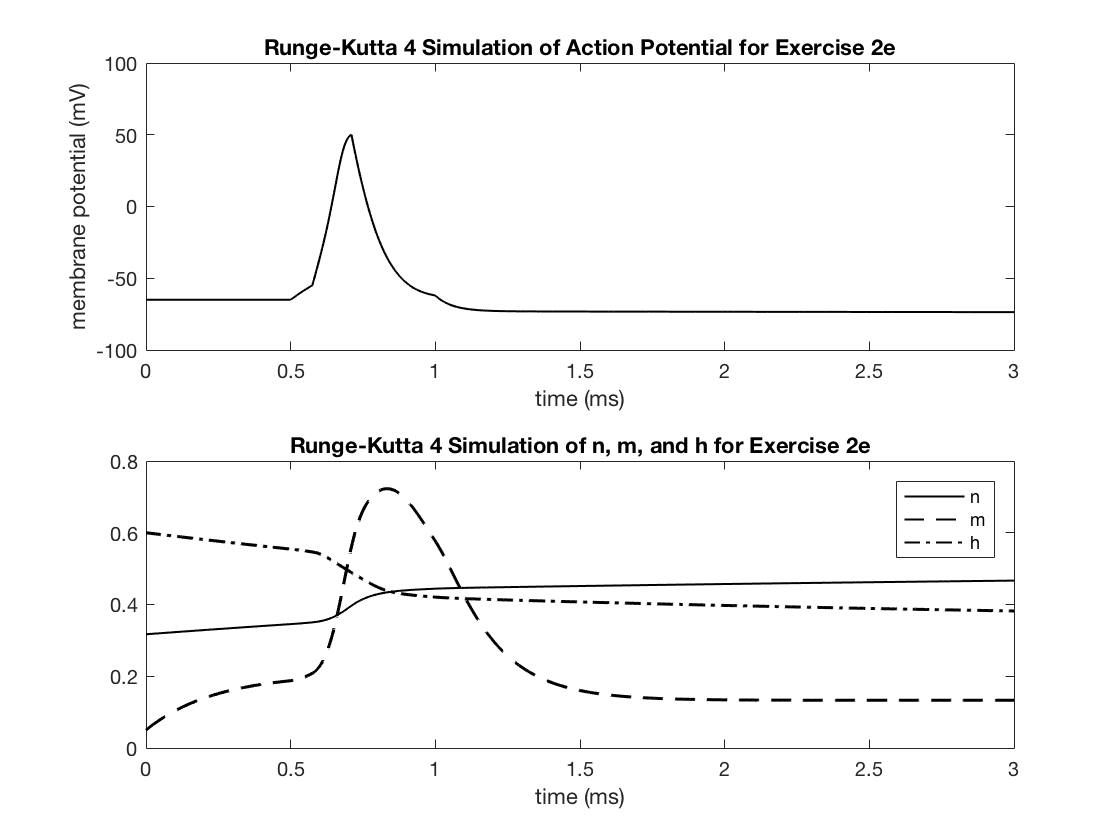
\includegraphics[width=0.666\textwidth]{2e-1}
  			 \centering
         \caption{Exercise 2e}
         \label{fig:2e-1}
       \end{figure}
				See Figure \ref{fig:2e-1}.
				
				This simulation looks the closest to the simulation in the book. By adding voltage gating to the leakage channel, the depolarization process happens faster, leading to an earlier repolarization phase. This creates a "pointy" tip to the action potential, similar to the graph in the book.
			
			\item
				One hypothesis for a way to increase the maximum action potential is to increase the displacement from the equilibrium potential for sodium. To test this, I increased the displacement constant in the simulation code and ran the simulation. Simply increasing this value did not increase the action potential, so I increased the voltage gating value for the sodium channel. Once I increased both of these values, the simulation was successfully able to increase the action potential.
			
		\end{enumerate}
  
\end{enumerate}

\end{document}